\documentclass[./answersheet.tex]{subfiles}

\begin{document}
\problem{16}
\begin{wts}
    Draw token bucket chart with $B=200$kb, and $r=2$Mbps, 5 bursts of \verb|300,400,250,200,20kb|
\end{wts}
\begin{proof}
    \verb|t = [0, 10, 20, 30, 40, 50, 60]|
    \verb|input_y = [0,300, 400, 250, 200, 20, 0]|
    \verb|bucket_y = [200,100,0,0,0,30,200]|
    \verb|output_y = [0,300,300,200,170,0,0]|
    \verb|queue_y = [0, 0,100, 150, 150, 0,0]|
    See the following graphics,\\
    % 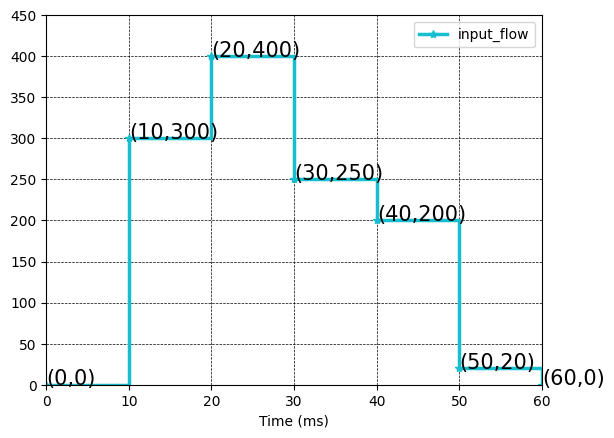
\includegraphics[width=0.5\linewidth]{./308_input_flow.png}
    % 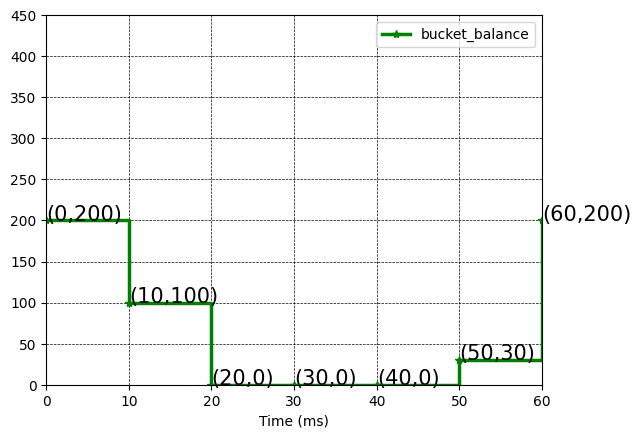
\includegraphics[width=.5\linewidth]{./308_bucket_balance.png}
    % 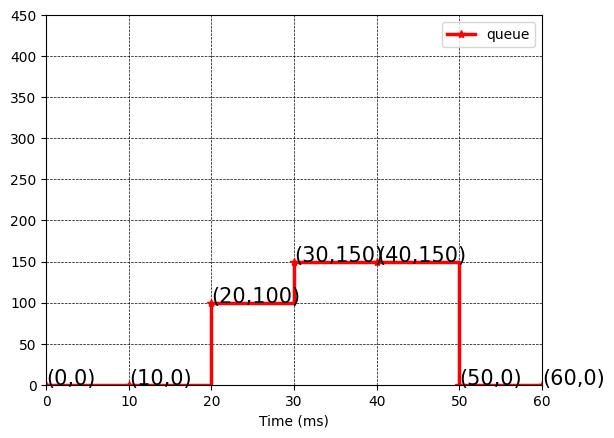
\includegraphics[width=.5\linewidth]{./308_queue.png}
    % 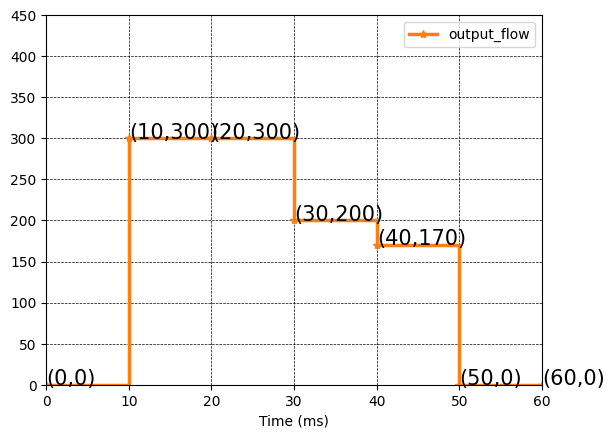
\includegraphics[width=.5\linewidth]{./308_output_flow.png}
    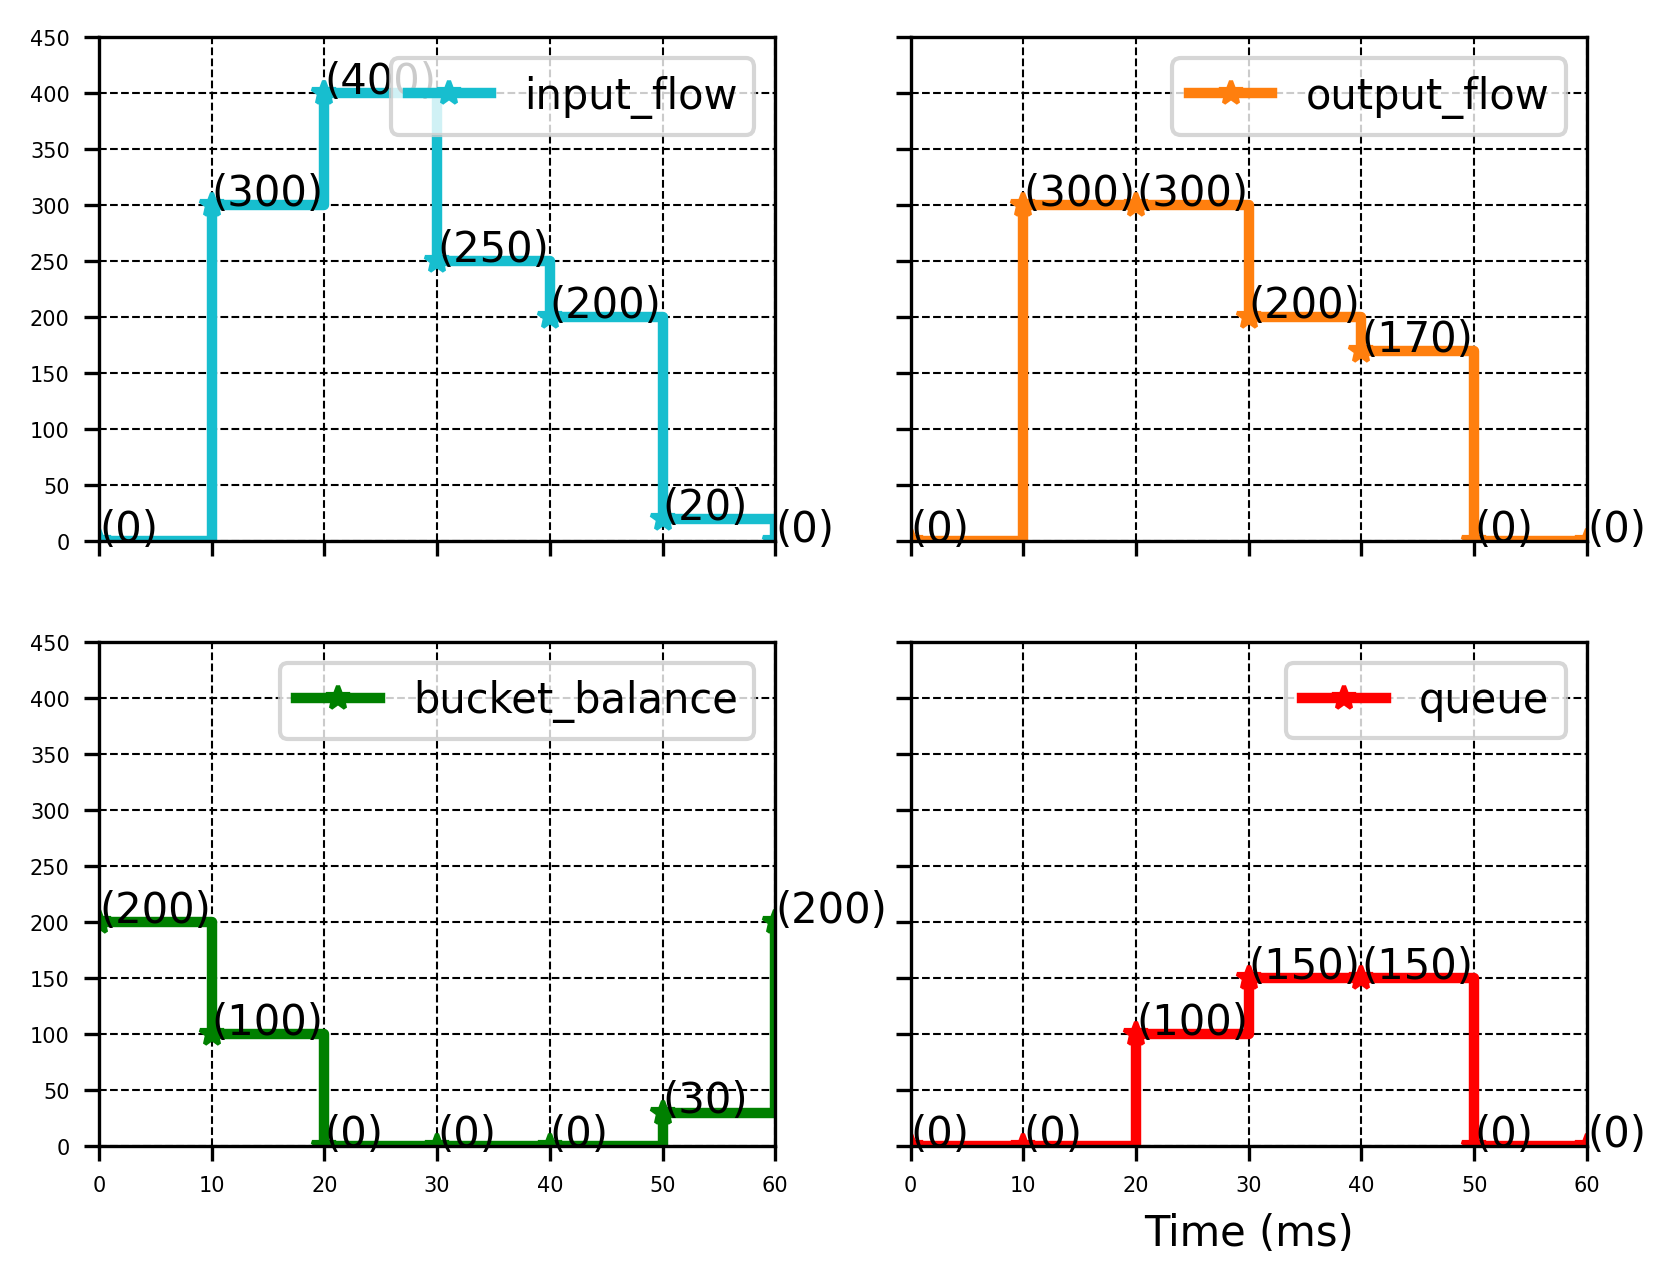
\includegraphics[width=\columnwidth]{./308_plots_all.png}
\end{proof}

\end{document}